% docs/latex/insertion-process.tex
\documentclass{standalone}
\usepackage{tikz}
\usetikzlibrary{arrows.meta,backgrounds,calc}

\begin{document}
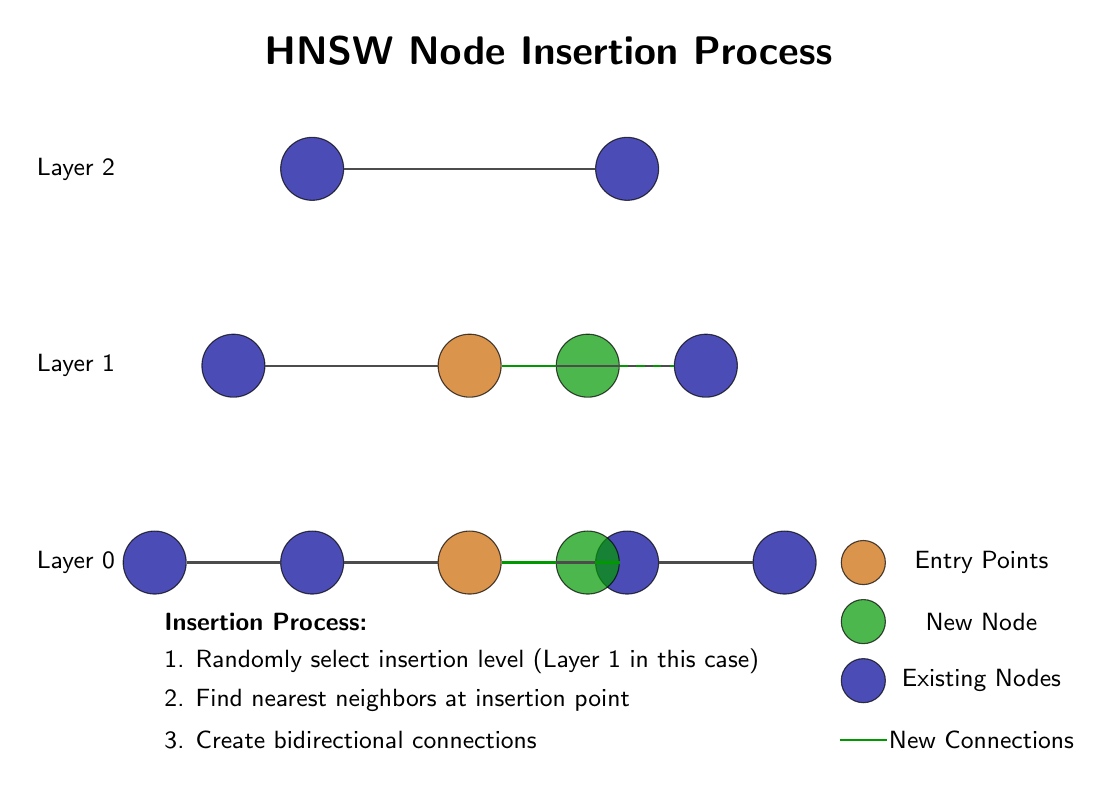
\begin{tikzpicture}[
    node/.style={circle, draw, fill=#1, minimum size=0.8cm, opacity=0.7},
    existing node/.style={node=blue!60!black},
    entry node/.style={node=orange!80!black},
    new node/.style={node=green!60!black},
    connection/.style={-, thick, gray!60!black},
    new connection/.style={-, thick, green!60!black},
    layer label/.style={font=\small\sffamily}
]

% Title
\node[font=\Large\sffamily\bfseries] at (1,4) {HNSW Node Insertion Process};

% Layer labels
\node[layer label] at (-5,2.5) {Layer 2};
\node[layer label] at (-5,0) {Layer 1};
\node[layer label] at (-5,-2.5) {Layer 0};

% Layer 2
\node[existing node] (L2N1) at (-2,2.5) {};
\node[existing node] (L2N2) at (2,2.5) {};
\draw[connection] (L2N1) -- (L2N2);

% Layer 1
\node[existing node] (L1N1) at (-3,0) {};
\node[entry node] (L1N2) at (0,0) {};
\node[existing node] (L1N3) at (3,0) {};
\node[new node] (L1New) at (1.5,0) {};
\draw[connection] (L1N1) -- (L1N2);
\draw[connection] (L1N2) -- (L1N3);
\draw[new connection] (L1N2) -- (L1New);
\draw[new connection, dashed] (L1New) -- (L1N3);

% Layer 0
\node[existing node] (L0N1) at (-4,-2.5) {};
\node[existing node] (L0N2) at (-2,-2.5) {};
\node[entry node] (L0N3) at (0,-2.5) {};
\node[existing node] (L0N4) at (2,-2.5) {};
\node[existing node] (L0N5) at (4,-2.5) {};
\node[new node] (L0New) at (1.5,-2.5) {};

\draw[connection] (L0N1) -- (L0N2);
\draw[connection] (L0N2) -- (L0N3);
\draw[connection] (L0N3) -- (L0N4);
\draw[connection] (L0N4) -- (L0N5);
\draw[new connection] (L0N3) -- (L0New);
\draw[new connection] (L0New) -- (L0N4);

% Legend
\begin{scope}[xshift=5cm, yshift=-4cm]
    \node[entry node, scale=0.7] at (0,1.5) {};
    \node[font=\small\sffamily] at (1.5,1.5) {Entry Points};
    
    \node[new node, scale=0.7] at (0,0.75) {};
    \node[font=\small\sffamily] at (1.5,0.75) {New Node};
    
    \node[existing node, scale=0.7] at (0,0) {};
    \node[font=\small\sffamily] at (1.5,0) {Existing Nodes};
    
    \draw[new connection] (-0.3,-0.75) -- (0.3,-0.75);
    \node[font=\small\sffamily] at (1.5,-0.75) {New Connections};
\end{scope}

% Process Steps
\begin{scope}[xshift=-4cm, yshift=-4.25cm]
    \node[font=\small\sffamily\bfseries, anchor=west] at (0,1) {Insertion Process:};
    \node[font=\small\sffamily, align=left, anchor=west] at (0,0.5) {1. Randomly select insertion level (Layer 1 in this case)};
    \node[font=\small\sffamily, align=left, anchor=west] at (0,0) {2. Find nearest neighbors at insertion point};
    \node[font=\small\sffamily, align=left, anchor=west] at (0,-0.5) {3. Create bidirectional connections};
\end{scope}

\end{tikzpicture}
\end{document}